\chapter{Géodésiques, accélération uniforme et limite newtonienne}

Le problème immédiat est celui de la gravité. Plus précisément, nous voulons déterminer la métrique de l’espace-temps qui décrit un champ gravitationnel presque uniforme, comme celui qui règne dans un petit laboratoire près de la surface de la Terre. Le chemin le plus court vers cette métrique se révèle indirect. Nous devons d’abord donner un sens opérationnel à trois idées géométriques : la dérivation covariante, le transport parallèle et le mouvement géodésique.

Ces idées sont liées. La dérivation covariante nous indique comment comparer des vecteurs en des points voisins. Le transport parallèle nous indique comment transporter un vecteur sans le faire tourner. Une géodésique est obtenue lorsque le vecteur transporté est lui-même tangent à la trajectoire. Dès que la trajectoire se trouve dans l’espace-temps plutôt que dans l’espace, cette même équation géodésique devient l’équation du mouvement d’une particule en chute libre.

La seconde moitié du cours opère ensuite un changement de perspective saisissant. Nous restons dans l’espace-temps plat de Minkowski, mais le décrivons au moyen de coordonnées adaptées à une famille d’observateurs en accélération rigide. Dans ces coordonnées, la métrique prend une allure gravitationnelle. Au voisinage d’un observateur, elle reproduit le potentiel d’un champ uniforme, et ses géodésiques obéissent à l’équation newtonienne
\begin{equation}
\frac{d^2y}{d\tau^2}=-g.
\end{equation}
C’est le principe d’équivalence exprimé par un calcul.

\section{Rappel sur la dérivée covariante}

En un point choisi \(P\), on peut sélectionner des coordonnées aussi cartésiennes que possible. Le cours emploie d’abord l’expression « coordonnées normales de Gauss », puis la précise aussitôt. Le nom importe moins que les conditions locales :
\begin{equation}
g_{mn}(P)=\delta_{mn},
\qquad
\partial_r g_{mn}(P)=0.
\label{eq:l4-normal-point}
\end{equation}
Ce sont des coordonnées normales en un point. Elles n’ont pas besoin de rester cartésiennes dans un voisinage fini, et il existe de nombreux repères de ce type, car on peut en faire tourner les axes.

La métrique est compatible avec l’opérateur de dérivation :
\begin{equation}
\nabla_r g_{mn}=0,
\qquad
\nabla_r g^{mn}=0.
\label{eq:l4-metric-compatibility}
\end{equation}
Pour un covecteur \(V_s\), la dérivée covariante est
\begin{equation}
\nabla_r V_s
=
\partial_r V_s-\Gamma^p{}_{rs}V_p.
\label{eq:l4-covector-derivative}
\end{equation}
Les coefficients de connexion sont
\begin{equation}
\Gamma^p{}_{rs}
=
\frac{1}{2}g^{pn}
\left(
\partial_s g_{nr}
+\partial_r g_{ns}
-\partial_n g_{rs}
\right).
\label{eq:l4-christoffel}
\end{equation}
Plusieurs indices sont corrigés au fur et à mesure que cette expression est écrite au tableau. L’équation \eqref{eq:l4-christoffel} est la relation achevée. Elle est symétrique en \(r\) et \(s\), comme il convient pour la connexion de Levi-Civita sans torsion.

\begin{figure}[htbp]
\centering
\includegraphics[width=0.92\textwidth]{lecture_04_figure_01.png}
\caption{Dérivée d’un covecteur et formule complète des symboles de Christoffel.}
\end{figure}

Puisque les symboles de Christoffel sont construits à partir des dérivées premières de la métrique, ils s’annulent en \(P\) dans les coordonnées \eqref{eq:l4-normal-point}. Ils ne s’annulent pas dans tous les systèmes de coordonnées, même lorsque l’espace sous-jacent est plat. Ainsi, \(\Gamma^p{}_{rs}\) n’est pas un tenseur. Ce caractère non tensoriel permettra précisément, plus tard, à un observateur accéléré de décrire une force gravitationnelle qu’un observateur inertiel ne voit pas.

\subsection{Relèvement de l’indice du vecteur}

On n’introduit pas la dérivée correspondante d’un vecteur comme une règle distincte à mémoriser. Elle découle de la métrique. Commençons par
\begin{equation}
V^n=g^{np}V_p.
\end{equation}
Alors
\begin{align}
\nabla_m V^n
&=\nabla_m\!\left(g^{np}V_p\right) \\
&=(\nabla_m g^{np})V_p+g^{np}\nabla_m V_p \\
&=g^{np}\left(\partial_mV_p-\Gamma^r{}_{mp}V_r\right),
\end{align}
où la compatibilité métrique a fait disparaître le premier terme. En réorganisant les indices, on obtient
\begin{equation}
\nabla_m V^n
=
\partial_m V^n+\Gamma^n{}_{mr}V^r.
\label{eq:l4-vector-derivative}
\end{equation}

\begin{figure}[htbp]
\centering
\includegraphics[width=0.90\textwidth]{lecture_04_figure_02.png}
\caption{Relèvement de l’indice au moyen de la métrique inverse avant la dérivation.}
\end{figure}

\begin{figure}[htbp]
\centering
\includegraphics[width=0.90\textwidth]{lecture_04_figure_03.png}
\caption{La dérivée à indice supérieur découle de la compatibilité métrique et de la règle du produit.}
\end{figure}

La règle des indices est donc simple :
\begin{equation}
\boxed{
\begin{aligned}
\text{lower index:}&\quad -\Gamma,\\
\text{upper index:}&\quad +\Gamma.
\end{aligned}}
\end{equation}
Pour un tenseur de rang supérieur, un terme de connexion intervient pour chaque indice, avec un signe déterminé par le fait que cet indice est inférieur ou supérieur.

\subsection{Question de terminologie}

Quelles sont exactement les meilleures coordonnées mentionnées plus haut ? On n’affirme pas qu’il s’agisse d’un système de coordonnées global privilégié. En un point choisi, elles donnent à la métrique sa forme plate et annulent ses dérivées premières. Une rotation des axes fournit un autre repère tout aussi valable. Les énoncés géométriques établis dans un tel repère ne dépendent pas de cette orientation, car les objets finaux sont des tenseurs.

\section{Transport parallèle le long d’une courbe}

Supposons qu’un vecteur \(V^n\) soit transporté le long d’une courbe. Pour un déplacement infinitésimal \(dx^m\), sa variation covariante est
\begin{align}
\delta V^n
&=(\nabla_mV^n)\,dx^m \\
&=\partial_mV^n\,dx^m
+\Gamma^n{}_{mr}V^r\,dx^m \\
&=dV^n+\Gamma^n{}_{mr}V^r\,dx^m.
\label{eq:l4-covariant-differential}
\end{align}

\begin{figure}[htbp]
\centering
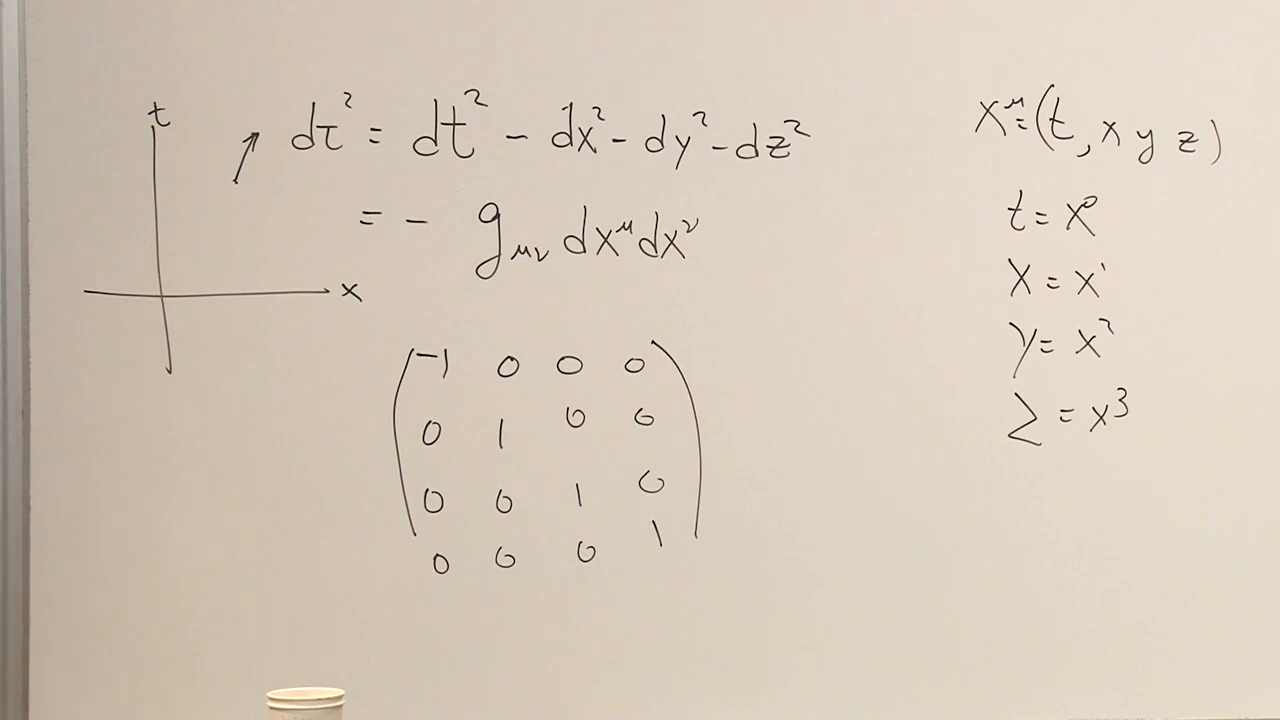
\includegraphics[width=0.92\textwidth]{lecture_04_figure_04.png}
\caption{La variation ordinaire des composantes et la correction de connexion le long d’une courbe.}
\end{figure}

Le vecteur est transporté parallèlement lorsque cette variation covariante s’annule :
\begin{equation}
\boxed{
dV^n+\Gamma^n{}_{mr}V^r\,dx^m=0.
}
\label{eq:l4-parallel-transport}
\end{equation}
Concrètement, on peut imaginer construire un repère normal en chaque point de la courbe. Dans ce repère local, le vecteur transporté ne doit pas tourner. On avance ensuite d’une distance infinitésimale, on construit le repère normal suivant et on recommence.

\begin{figure}[htbp]
\centering
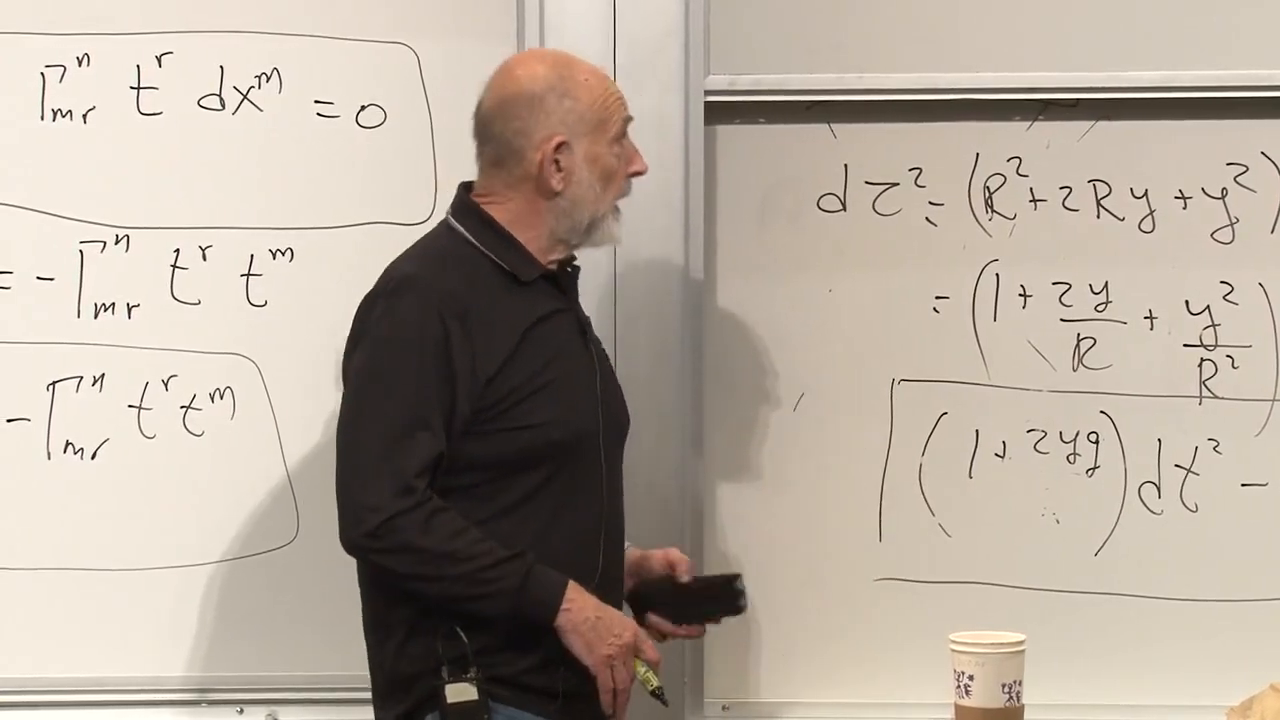
\includegraphics[width=0.92\textwidth]{lecture_04_figure_05.png}
\caption{Écriture claire de l’équation du transport parallèle au tableau.}
\end{figure}

L’orientation de chaque repère normal temporaire ne fait pas partie de la physique. On pourrait le faire tourner avant d’effectuer la comparaison. Ce qui compte, c’est que l’énoncé covariant \eqref{eq:l4-parallel-transport} soit indépendant de ce choix arbitraire.

\subsection{Dépendance au chemin et courbure}

Dans un espace courbe, le transport parallèle dépend du chemin. Partons du même vecteur au même point initial et transportons-le jusqu’au même point final en suivant deux chemins différents. En général, les vecteurs finaux diffèrent. Un vecteur transporté le long d’une boucle fermée peut revenir tourné. Cette différence est l’holonomie et constitue un signe direct de courbure.

\begin{figure}[htbp]
\centering
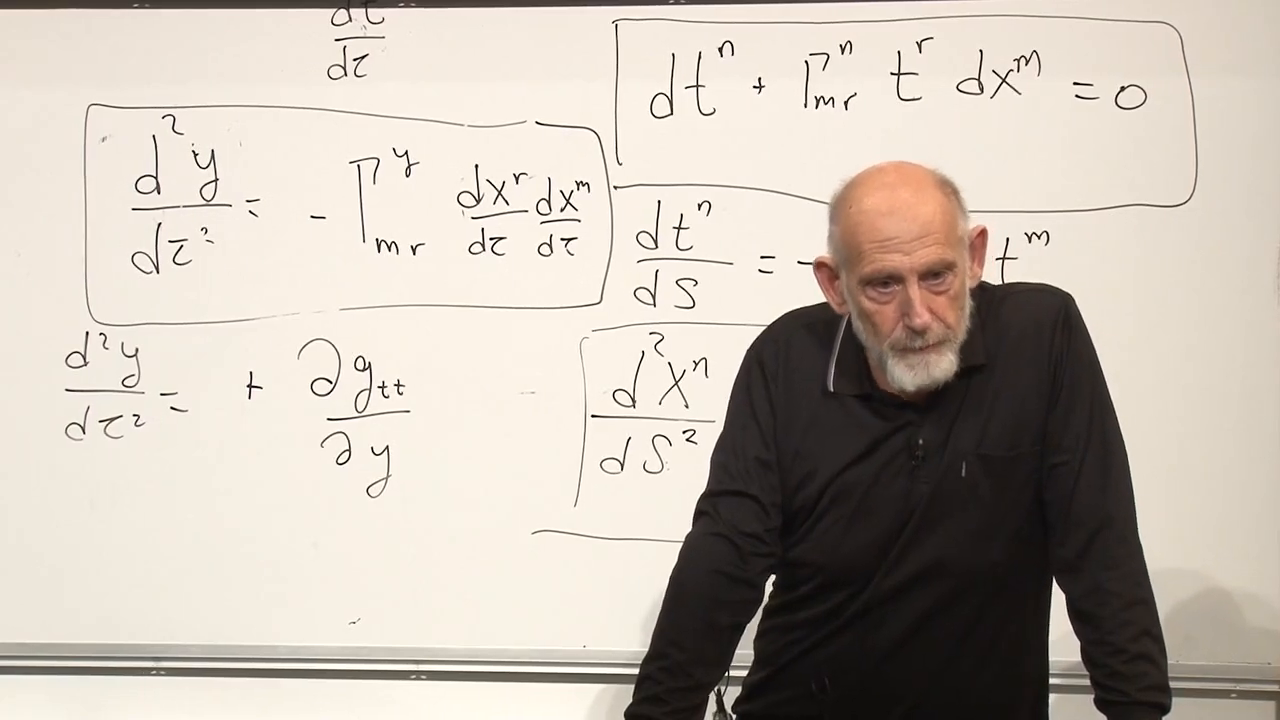
\includegraphics[width=0.90\textwidth]{lecture_04_figure_06.png}
\caption{Sur une surface courbe, deux chemins ne transportent pas nécessairement un vecteur selon la même orientation finale.}
\end{figure}

Le cône fournit un exemple utile. À l’écart de sa pointe, on peut découper un cône et l’aplatir. Pourtant, après le transport parallèle le long d’une boucle qui entoure la pointe, le vecteur revient tourné de l’angle de défaut. Si la pointe est arrondie, la courbure est finie et répartie sur une petite région. Si elle est parfaitement aiguë, l’idéalisation concentre la courbure en ce point.

\begin{figure}[htbp]
\centering
\includegraphics[width=0.90\textwidth]{lecture_04_figure_07.png}
\caption{Mouvement circulaire sur le cône et représentation plane après découpe.}
\end{figure}

\subsection{Questions sur le vecteur transporté}

\paragraph{Le vecteur doit-il être défini partout ?}
Non. On peut partir d’un seul vecteur en un point et résoudre \eqref{eq:l4-parallel-transport} uniquement le long de la courbe choisie. Un champ vectoriel complet est facultatif. Si un champ est défini sur une région, il peut être covariantement constant dans une direction et ne pas l’être dans une autre.

\paragraph{Sa norme est-elle conservée ?}
Oui. Posons \(V^2=g_{mn}V^mV^n\). Le long de la courbe,
\begin{align}
\frac{D}{d\lambda}\left(g_{mn}V^mV^n\right)
&=
\frac{Dg_{mn}}{d\lambda}V^mV^n
+2g_{mn}V^m\frac{DV^n}{d\lambda}\\
&=0.
\end{align}
La compatibilité métrique annule le premier terme et le transport parallèle annule le second. Les normes et les angles mutuels des vecteurs transportés parallèlement sont donc conservés.

\paragraph{Le vecteur tangent à toute courbe est-il transporté parallèlement ?}
Non. Cette question mène directement aux géodésiques. Le vecteur tangent à un chemin circulaire autour d’un cône tourne continuellement. Celui de la droite obtenue en découpant le cône ne tourne pas. Seul le second chemin est localement rectiligne.

\section{Géodésiques : le chemin le plus droit, pas seulement le plus court}

Une géodésique admet deux descriptions liées. Globalement, c’est un chemin stationnaire pour la fonctionnelle de longueur ou de temps propre. Localement, c’est le chemin le plus droit possible. Le mot « stationnaire » est important : selon la géométrie et les extrémités considérées, le chemin n’est pas forcément l’unique minimum global. Dans l’espace-temps lorentzien, les géodésiques de genre temps maximisent localement le temps propre plutôt que de minimiser une distance positive.

C’est la description locale qui nous est utile ici. Une petite voiture roulant sur un terrain courbe, avec le volant maintenu droit devant, suit une géodésique, à condition que sa taille soit petite devant l’échelle à laquelle le terrain se courbe. Sa trajectoire n’a pas besoin de paraître droite dans un espace ambiant : elle est droite selon la géométrie définie sur la surface.

\begin{figure}[htbp]
\centering
\includegraphics[width=0.90\textwidth]{lecture_04_figure_08.png}
\caption{Trajectoire tracée intrinsèquement sur la surface courbe, pour introduire la définition du chemin le plus droit.}
\end{figure}

\subsection{Le vecteur tangent}

Soit la courbe \(x^m(s)\), de longueur d’arc
\begin{equation}
ds^2=g_{mn}\,dx^m dx^n.
\end{equation}
Son vecteur tangent unitaire est
\begin{equation}
t^m=\frac{dx^m}{ds}.
\label{eq:l4-unit-tangent}
\end{equation}
Géométriquement, prenons deux points voisins, formons le vecteur déplacement qui les relie, divisons-le par leur distance, puis faisons coïncider les deux points.

\begin{figure}[htbp]
\centering
\includegraphics[width=0.90\textwidth]{lecture_04_figure_09.png}
\caption{La direction tangente comme limite du déplacement le long d’une courbe.}
\end{figure}

\begin{figure}[htbp]
\centering
\includegraphics[width=0.90\textwidth]{lecture_04_figure_10.png}
\caption{Élément de ligne et vecteur tangent unitaire \(t^m=dx^m/ds\).}
\end{figure}

Une géodésique est une courbe dont le vecteur tangent est transporté parallèlement le long de la courbe elle-même :
\begin{equation}
dt^n+\Gamma^n{}_{mr}t^r\,dx^m=0.
\end{equation}
Divisons par \(ds\) et utilisons \(dx^m/ds=t^m\) :
\begin{equation}
\frac{dt^n}{ds}
=
-\Gamma^n{}_{mr}t^m t^r.
\end{equation}
Enfin, substituons \(t^n=dx^n/ds\) :
\begin{equation}
\boxed{
\frac{d^2x^n}{ds^2}
+\Gamma^n{}_{mr}
\frac{dx^m}{ds}
\frac{dx^r}{ds}
=0.
}
\label{eq:l4-geodesic}
\end{equation}

\begin{figure}[htbp]
\centering
\includegraphics[width=0.94\textwidth]{lecture_04_figure_11.png}
\caption{Loi de transport du vecteur tangent et équation géodésique du second ordre.}
\end{figure}

L’équation \eqref{eq:l4-geodesic} ressemble déjà à la dynamique newtonienne. Si l’on remplace \(s\) par un paramètre de temps approprié, le premier terme est une accélération. Le terme de connexion joue alors le rôle d’une force par unité de masse, entièrement déterminée par la métrique. En relativité générale, cette analogie devient littérale : les particules libres suivent des géodésiques de l’espace-temps, et ce que Newton appelait l’accélération gravitationnelle apparaît par l’intermédiaire de la connexion.

\section{De la distance riemannienne au temps propre de l’espace-temps}

La discussion passe maintenant de l’espace courbe à l’espace-temps. Dans des coordonnées cartésiennes inertielles, le temps propre entre des événements voisins est
\begin{equation}
d\tau^2
=dt^2-dx^2-dy^2-dz^2.
\label{eq:l4-proper-time}
\end{equation}
Le cours utilise
\begin{equation}
d\tau^2=-g_{\mu\nu}\,dx^\mu dx^\nu
\label{eq:l4-lecture-sign}
\end{equation}
avec
\begin{equation}
g_{\mu\nu}
=
\eta_{\mu\nu}
=
\begin{pmatrix}
-1&0&0&0\\
0&1&0&0\\
0&0&1&0\\
0&0&0&1
\end{pmatrix}.
\label{eq:l4-eta}
\end{equation}
Le signe moins extérieur dans \eqref{eq:l4-lecture-sign} convertit donc la métrique choisie, de signature principalement positive, en \eqref{eq:l4-proper-time}. Les coordonnées sont
\begin{equation}
\begin{aligned}
x^\mu&=(t,x,y,z),\\
x^0&=t,\quad x^1=x,\\
x^2&=y,\quad x^3=z.
\end{aligned}
\end{equation}

\begin{figure}[htbp]
\centering
\includegraphics[width=0.94\textwidth]{lecture_04_figure_12.png}
\caption{Temps propre, coordonnées de l’espace-temps et métrique de Minkowski à signature principalement positive.}
\end{figure}

L’information invariante est la signature : une valeur propre a le signe associé au temps et trois ont celui associé à l’espace. Multiplier la métrique entière par \(-1\) et ajuster toutes les conventions de façon cohérente donne la convention tout aussi courante à signature principalement négative. Aucun phénomène physique ne dépend de ce choix global.

Le cours demande si l’on a envisagé des espaces ayant d’autres signatures indéfinies. Mathématiquement, les géométries pseudo-riemanniennes de nombreuses signatures sont bien établies. Le point physique est plus restreint : l’espace-temps relativiste observé est lorentzien, avec une direction temporelle. Des directions temporelles supplémentaires modifieraient profondément la structure causale et ne décrivent pas la physique examinée ici.

\begin{figure}[htbp]
\centering
\includegraphics[width=0.94\textwidth]{lecture_04_figure_13.png}
\caption{La convention de signe est vérifiée avant que la métrique plate soit notée \(\eta_{\mu\nu}\).}
\end{figure}

Un espace-temps plat n’exige pas que les composantes de la métrique aient l’allure de \(\eta_{\mu\nu}\) dans tous les systèmes de coordonnées. Cela signifie qu’il existe des coordonnées dans lesquelles elles l’ont. Des coordonnées curvilignes ou accélérées peuvent faire varier les composantes avec la position, même si le tenseur de Riemann est nul.

\section{Pourquoi une même accélération des coordonnées ne donne pas un système rigide}

Nous voulons construire des coordonnées liées à un ascenseur en accélération. La première idée consiste à aligner plusieurs observateurs à des distances fixes et à leur donner à tous la même accélération coordonnée. La relativité empêche cette construction naïve de rester rigide.

\begin{figure}[htbp]
\centering
\includegraphics[width=0.92\textwidth]{lecture_04_figure_14.png}
\caption{Alignement d’observateurs voisins pour vérifier si une accélération commune préserve la rigidité.}
\end{figure}

Si, dans un même repère inertiel, des observateurs séparés suivent des programmes d’accélération identiques, leur distance ne reste pas fixe dans leurs repères de repos instantanés changeants. Une corde qui les relie s’étire et finit par rompre. C’est la même tension cinématique que celle mise en évidence par l’expérience de pensée des vaisseaux de Bell. De plus, une accélération coordonnée newtonienne constante ne peut se poursuivre indéfiniment : elle finirait par prédire une vitesse supérieure à celle de la lumière.

Un repère accéléré rigide au sens relativiste doit donc appliquer une accélération propre différente à chaque position. Les observateurs plus proches de l’horizon auquel on s’approche accélèrent davantage ; ceux qui en sont plus éloignés accélèrent moins. Leurs distances propres peuvent alors rester constantes dans le repère comobile à l’instant considéré. Il s’agit d’une accélération rigide au sens de Born dans une dimension spatiale.

\section{Les coordonnées polaires euclidiennes : un préalable}

La construction correcte apparaît plus facilement si l’on commence par un cercle ordinaire. Dans un plan euclidien,
\begin{equation}
x=r\cos\theta,
\qquad
y=r\sin\theta,
\end{equation}
d’où
\begin{equation}
x^2+y^2=r^2,
\qquad
\cos^2\theta+\sin^2\theta=1.
\end{equation}
Les expressions faisant intervenir l’exponentielle complexe sont
\begin{equation}
\cos\theta=\frac{e^{i\theta}+e^{-i\theta}}{2},
\qquad
\sin\theta=\frac{e^{i\theta}-e^{-i\theta}}{2i}.
\label{eq:l4-euler-trig}
\end{equation}
Lors de la discussion au tableau, on remarque qu’il manque le facteur \(i\) au dénominateur de la formule du sinus, puis on le rétablit.

\begin{figure}[htbp]
\centering
\includegraphics[width=0.94\textwidth]{lecture_04_figure_15.png}
\caption{Cercle, coordonnées polaires euclidiennes et formes exponentielles des fonctions trigonométriques.}
\end{figure}

Une valeur fixe de \(r\) définit un cercle. Un mouvement à vitesse angulaire constante a une accélération centripète de norme constante, toujours dirigée vers l’intérieur. L’hyperbole jouera le rôle correspondant dans l’espace-temps.

\section{Coordonnées hyperboliques dans l’espace-temps de Minkowski}

Remplaçons les fonctions trigonométriques par leurs analogues hyperboliques :
\begin{equation}
\cosh\omega=\frac{e^\omega+e^{-\omega}}{2},
\qquad
\sinh\omega=\frac{e^\omega-e^{-\omega}}{2},
\end{equation}
avec
\begin{equation}
\cosh^2\omega-\sinh^2\omega=1.
\label{eq:l4-hyperbolic-identity}
\end{equation}
Il n’y a pas de facteur \(i\). La coordonnée \(\omega\) est un angle hyperbolique, ou rapidité. Contrairement à un angle ordinaire, elle n’est pas périodique ; elle varie de \(-\infty\) à \(+\infty\).

\begin{figure}[htbp]
\centering
\includegraphics[width=0.94\textwidth]{lecture_04_figure_16.png}
\caption{Dans la construction de l’espace-temps, les fonctions circulaires sont remplacées par les fonctions hyperboliques.}
\end{figure}

Définissons de nouvelles coordonnées dans le secteur de Rindler droit :
\begin{equation}
x=r\cosh\omega,
\qquad
t=r\sinh\omega,
\qquad
r>0.
\label{eq:l4-rindler-transform}
\end{equation}
Alors
\begin{equation}
x^2-t^2=r^2.
\label{eq:l4-rindler-hyperbola}
\end{equation}
À \(r\) fixe, la variation de \(\omega\) décrit une hyperbole. Faire croître \(r\) déplace d’une hyperbole à l’autre dans une direction de genre espace, tandis que faire croître \(\omega\) fait avancer le long d’une hyperbole, dans une direction de genre temps.

\begin{figure}[htbp]
\centering
\includegraphics[width=0.94\textwidth]{lecture_04_figure_17.png}
\caption{Transformation de coordonnées \(x=r\cosh\omega\), \(t=r\sinh\omega\) et hyperbole invariante correspondante.}
\end{figure}

\begin{figure}[htbp]
\centering
\includegraphics[width=0.94\textwidth]{lecture_04_figure_18.png}
\caption{Famille d’hyperboles à \(r\) fixe représentant un ensemble d’observateurs en accélération rigide.}
\end{figure}

\subsection{La métrique en coordonnées accélérées}

Dérivons \eqref{eq:l4-rindler-transform} :
\begin{align}
dx&=\cosh\omega\,dr+r\sinh\omega\,d\omega,\\
dt&=\sinh\omega\,dr+r\cosh\omega\,d\omega.
\end{align}
En utilisant \eqref{eq:l4-hyperbolic-identity}, les termes croisés s’annulent :
\begin{align}
d\tau^2
&=dt^2-dx^2\\
&=r^2\,d\omega^2-dr^2.
\label{eq:l4-rindler-metric}
\end{align}
Une fois les directions transversales rétablies, elles ajoutent simplement \(-dy^2-dz^2\) à la convention de temps propre utilisée ici.

Il s’agit toujours d’un espace-temps plat. Le coefficient dépendant des coordonnées \(r^2\) n’indique pas plus une courbure que le facteur \(r^2\) devant \(d\theta^2\) dans les coordonnées polaires euclidiennes.

\subsection{Accélération propre le long des hyperboles}

Pour une ligne d’univers fixe \(r=R\), l’équation \eqref{eq:l4-rindler-metric} donne
\begin{equation}
d\tau=R\,d\omega.
\end{equation}
Sa quadrivitesse est
\begin{equation}
U^\mu
=
\frac{d(t,x)}{d\tau}
=
(\cosh\omega,\sinh\omega),
\end{equation}
et sa quadriaccélération est
\begin{equation}
A^\mu
=
\frac{dU^\mu}{d\tau}
=
\frac{1}{R}(\sinh\omega,\cosh\omega).
\end{equation}
Sa norme invariante est constante :
\begin{equation}
a=\sqrt{A^\mu A_\mu}=\frac{1}{R}
\qquad (c=1).
\label{eq:l4-proper-acceleration}
\end{equation}

\begin{figure}[htbp]
\centering
\includegraphics[width=0.90\textwidth]{lecture_04_figure_19.png}
\caption{Loi en raison inverse \(a=1/R\) pour une ligne d’univers accélérée fixe.}
\end{figure}

En rétablissant les unités,
\begin{equation}
\boxed{a=\frac{c^2}{R}.}
\label{eq:l4-proper-acceleration-units}
\end{equation}

\begin{figure}[htbp]
\centering
\includegraphics[width=0.90\textwidth]{lecture_04_figure_20.png}
\caption{Le rétablissement des unités transforme \(1/R\) en \(c^2/R\).}
\end{figure}

Plus l’interception \(R\) est petite, plus la ligne d’univers se courbe fortement et plus l’accélération propre ressentie par l’observateur est grande. Les hyperboles plus éloignées se courbent moins et exigent une accélération plus faible. Chaque observateur a une accélération constante au cours du temps, mais les accélérations diffèrent d’un observateur à l’autre. C’est précisément cette variation qui préserve les distances propres entre eux.

\subsection{Questions sur les coordonnées accélérées}

\paragraph{\(R\) est-il l’intercept selon \(x\) ?}
Oui. Pour \(\omega=0\), l’équation \eqref{eq:l4-rindler-transform} donne \(t=0\) et \(x=R\). L’intercept détermine l’accélération propre par \eqref{eq:l4-proper-acceleration-units}.

\paragraph{La construction dépend-elle de l’origine choisie ?}
Les coordonnées en dépendent. Une translation de l’origine produit une autre famille d’hyperboles, dont les asymptotes sont déplacées. Aucun phénomène physique invariant ne dépend de ce choix. Nous sélectionnons délibérément un système de coordonnées accéléré et cherchons à savoir comment le mouvement inertiel s’y décrit.

\paragraph{Qu’est-ce que l’accélération propre ?}
C’est l’accélération mesurée par un accéléromètre solidaire de l’observateur. Covariamment,
\begin{equation}
A^\mu=\frac{dU^\mu}{d\tau},
\qquad
U^\mu=\frac{dx^\mu}{d\tau}.
\end{equation}
Sa norme est la poussée effectivement ressentie par l’observateur, et non l’accélération coordonnée \(d^2x/dt^2\) attribuée par un repère distant.

\section{Métriques plates en coordonnées polaires et hyperboliques}

Avant de nous placer au voisinage de la Terre, il est utile de mettre côte à côte les métriques euclidienne et lorentzienne. Dans le plan,
\begin{equation}
ds^2=dr^2+r^2d\theta^2,
\qquad
g_{ab}
=
\begin{pmatrix}
1&0\\
0&r^2
\end{pmatrix}.
\label{eq:l4-polar-metric}
\end{equation}
Une suggestion de l’auditoire introduit brièvement un facteur sphérique, mais il s’agit d’un plan, pas d’une sphère. Le terme \(r^2\) traduit le fait qu’un intervalle angulaire donné couvre un arc plus long à plus grand rayon.

\begin{figure}[htbp]
\centering
\includegraphics[width=0.94\textwidth]{lecture_04_figure_21.png}
\caption{Métrique polaire euclidienne : composantes dépendant de la position dans un plan plat.}
\end{figure}

L’analogue de Minkowski est
\begin{equation}
d\tau^2=r^2d\omega^2-dr^2.
\end{equation}
Les deux métriques ont des composantes qui dépendent de la position, alors que les deux géométries sont plates. La courbure des coordonnées et la courbure géométrique sont deux choses différentes.

\section{Localisation au voisinage de l’accélération terrestre}

Choisissons une hyperbole de référence dont l’accélération propre est égale à la valeur terrestre \(g\) :
\begin{equation}
g=\frac{c^2}{R},
\qquad
R=\frac{c^2}{g}.
\label{eq:l4-earth-radius}
\end{equation}

\begin{figure}[htbp]
\centering
\includegraphics[width=0.94\textwidth]{lecture_04_figure_22.png}
\caption{Choix de l’hyperbole de référence au moyen de \(c^2/R=g\).}
\end{figure}

Numériquement,
\begin{equation}
R
\simeq
\frac{(3.0\times10^8\ {\rm m\,s^{-1}})^2}
{9.8\ {\rm m\,s^{-2}}}
\simeq
9.2\times10^{15}\ {\rm m}.
\end{equation}
Le cours arrondit cette valeur à \(10^{16}\) mètres. Un champ d’un \(g\) terrestre est modeste à l’échelle relativiste ; le rayon de Rindler correspondant est donc immense.

Examinons maintenant un petit voisinage seulement de cet observateur de référence. Introduisons une hauteur locale \(y\) définie par
\begin{equation}
r=R+y,
\qquad
dr=dy,
\qquad
|y|\ll R.
\label{eq:l4-local-height}
\end{equation}
L’égalité \(dr=dy\) est explicitement repérée pendant la discussion ; le terme spatial doit donc s’écrire \(-dy^2\).

La substitution dans \eqref{eq:l4-rindler-metric} donne
\begin{align}
d\tau^2
&=(R+y)^2d\omega^2-dy^2\\
&=(R^2+2Ry+y^2)d\omega^2-dy^2\\
&=
\left(
1+\frac{2y}{R}+\frac{y^2}{R^2}
\right)
R^2d\omega^2-dy^2.
\label{eq:l4-local-expand}
\end{align}

\begin{figure}[htbp]
\centering
\includegraphics[width=0.94\textwidth]{lecture_04_figure_23.png}
\caption{Développement de la métrique accélérée au voisinage de \(r=R+y\).}
\end{figure}

Définissons une coordonnée de temps local
\begin{equation}
t=R\omega.
\label{eq:l4-local-time}
\end{equation}
Alors
\begin{equation}
d\tau^2
=
\left(
1+\frac{2y}{R}+\frac{y^2}{R^2}
\right)dt^2-dy^2.
\label{eq:l4-local-exact}
\end{equation}

\begin{figure}[htbp]
\centering
\includegraphics[width=0.94\textwidth]{lecture_04_figure_24.png}
\caption{Introduction de \(t=R\omega\) après le développement autour de l’hyperbole de référence.}
\end{figure}

Même un déplacement vertical de plusieurs dizaines de kilomètres est minuscule devant \(R\). Pour rendre la comparaison parlante, le cours considère une chute d’environ vingt-quatre miles : cette distance reste négligeable devant \(10^{16}\) mètres. Par conséquent, \(y^2/R^2\) est beaucoup plus petit que \(y/R\), et l’on peut négliger le terme quadratique :
\begin{equation}
d\tau^2
\simeq
\left(1+\frac{2y}{R}\right)dt^2-dy^2.
\label{eq:l4-local-linear}
\end{equation}

\begin{figure}[htbp]
\centering
\includegraphics[width=0.94\textwidth]{lecture_04_figure_25.png}
\caption{Métrique développée et changement de variable pour le temps local avant la troncature en champ faible.}
\end{figure}

Dans les unités où \(c=1\), l’équation \eqref{eq:l4-earth-radius} donne \(1/R=g\), et donc
\begin{equation}
\boxed{
d\tau^2\simeq(1+2gy)\,dt^2-dy^2.
}
\label{eq:l4-uniform-metric}
\end{equation}

\begin{figure}[htbp]
\centering
\includegraphics[width=0.94\textwidth]{lecture_04_figure_26.png}
\caption{Métrique locale complète de l’ascenseur en accélération uniforme.}
\end{figure}

La quantité
\begin{equation}
\Phi(y)=gy
\end{equation}
est le potentiel gravitationnel newtonien par unité de masse dans un champ uniforme. Ainsi,
\begin{equation}
d\tau^2\simeq(1+2\Phi)\,dt^2-dy^2
\qquad (c=1).
\label{eq:l4-weak-potential-propertime}
\end{equation}
Avec la convention du cours \(d\tau^2=-g_{\mu\nu}dx^\mu dx^\nu\), cela signifie que
\begin{equation}
g_{tt}=-(1+2\Phi).
\label{eq:l4-gtt-potential}
\end{equation}
En unités conventionnelles, la correction sans dimension est \(2\Phi/c^2\).

L’espace-temps n’a subi aucune courbure. L’équation \eqref{eq:l4-uniform-metric} est le développement local d’une métrique plate de Rindler. La gravité apparente est la force d’inertie ressentie dans un ascenseur accéléré.

\section{L’équation géodésique devient la loi de Newton}

Jusqu’ici, l’identification de \(gy\) à un potentiel n’était qu’une suggestion. Le test décisif est dynamique : une particule libre dans la métrique \eqref{eq:l4-uniform-metric} accélère-t-elle vers le bas avec \(d^2y/dt^2=-g\) ?

Pour une ligne d’univers de genre temps paramétrée par le temps propre,
\begin{equation}
\frac{d^2x^\nu}{d\tau^2}
+\Gamma^\nu{}_{\mu\rho}
\frac{dx^\mu}{d\tau}
\frac{dx^\rho}{d\tau}
=0.
\label{eq:l4-spacetime-geodesic}
\end{equation}
La composante verticale est
\begin{equation}
\frac{d^2y}{d\tau^2}
=
-\Gamma^y{}_{\mu\rho}
\frac{dx^\mu}{d\tau}
\frac{dx^\rho}{d\tau}.
\label{eq:l4-y-geodesic}
\end{equation}

\begin{figure}[htbp]
\centering
\includegraphics[width=0.94\textwidth]{lecture_04_figure_27.png}
\caption{Équation de transport et sa forme géodésique du second ordre, prêtes à être appliquées au mouvement vertical.}
\end{figure}

\subsection{Approximation des faibles vitesses}

Pour une particule se déplaçant lentement dans un champ faible et statique,
\begin{equation}
\frac{dt}{d\tau}\simeq1,
\qquad
\left|\frac{dy}{d\tau}\right|\ll1.
\end{equation}
La composante temporelle de la quadrivitesse est donc de l’ordre de l’unité, tandis que les composantes spatiales sont petites devant elle. Parmi les produits de \eqref{eq:l4-y-geodesic}, le terme dominant correspond à \(\mu=\rho=t\) :
\begin{equation}
\frac{d^2y}{d\tau^2}
\simeq
-\Gamma^y{}_{tt}
\left(\frac{dt}{d\tau}\right)^2
\simeq
-\Gamma^y{}_{tt}.
\label{eq:l4-slow-geodesic}
\end{equation}

\begin{figure}[htbp]
\centering
\includegraphics[width=0.94\textwidth]{lecture_04_figure_28.png}
\caption{Spécialisation de l’équation géodésique de l’espace-temps à la composante \(y\) pour un mouvement lent.}
\end{figure}

Calculons maintenant le seul coefficient de connexion nécessaire. La métrique est diagonale et indépendante de \(t\), donc
\begin{align}
\Gamma^y{}_{tt}
&=
\frac{1}{2}g^{yy}
\left(
\partial_tg_{yt}
+\partial_tg_{ty}
-\partial_yg_{tt}
\right)\\
&=
-\frac{1}{2}\partial_yg_{tt},
\label{eq:l4-gamma-ytt}
\end{align}
car \(g^{yy}=1\) dans la convention tensorielle à signature principalement positive du cours.

\begin{figure}[htbp]
\centering
\includegraphics[width=0.94\textwidth]{lecture_04_figure_29.png}
\caption{Formule de Christoffel réduite à la composante \(y,t,t\).}
\end{figure}

En combinant \eqref{eq:l4-slow-geodesic} et \eqref{eq:l4-gamma-ytt},
\begin{equation}
\frac{d^2y}{d\tau^2}
\simeq
\frac{1}{2}\partial_yg_{tt}.
\label{eq:l4-accel-gtt}
\end{equation}
D’après \eqref{eq:l4-gtt-potential},
\begin{equation}
\partial_yg_{tt}
=
-2\partial_y\Phi
=
-2g.
\end{equation}
Par conséquent,
\begin{equation}
\boxed{
\frac{d^2y}{d\tau^2}=-g.
}
\label{eq:l4-newton-result}
\end{equation}
Comme \(t\simeq\tau\) dans la même approximation de faible vitesse, on obtient aussi
\begin{equation}
\frac{d^2y}{dt^2}=-g.
\end{equation}

\begin{figure}[htbp]
\centering
\includegraphics[width=0.94\textwidth]{lecture_04_figure_30.png}
\caption{Enchaînement complet des signes : la dérivée par rapport à \(y\) de \(g_{tt}\) donne l’accélération \(-g\).}
\end{figure}

Plus généralement, dans le régime newtonien,
\begin{equation}
\boxed{
\begin{aligned}
g_{tt}&=-(1+2\Phi),\\
\frac{d^2x^i}{dt^2}&=-\partial_i\Phi
\end{aligned}
}
\qquad(c=1).
\label{eq:l4-newton-general}
\end{equation}
Lorsque les unités sont rétablies, la correction métrique est \(2\Phi/c^2\), tandis que l’accélération reste \(-\boldsymbol{\nabla}\Phi\).

Ce calcul explique pourquoi la métrique, plutôt qu’un champ de force gravitationnelle distinct, est l’objet central. Une particule libre suit simplement une géodésique de l’espace-temps. Dans des coordonnées adaptées à un laboratoire accéléré, cette géodésique présente la courbure coordonnée habituellement attribuée à la gravité.

\subsection{Question sur l’origine de Rindler choisie}

Aurait-on pu décaler l’hyperbole de référence, de sorte que ses asymptotes et son intercept se trouvent ailleurs ? Oui. Il existe un système de coordonnées à accélération uniforme associé à toute origine translatée adéquate. Dans l’image de l’ascenseur, ces choix reviennent à sélectionner des ascenseurs dont les planchers occupent des positions différentes à un instant donné.

Le résultat local ne repose pas sur une origine privilégiée. Une fois choisi un observateur de référence d’accélération \(g\), \(y\) mesure la hauteur par rapport à cet observateur et la métrique voisine prend la forme \eqref{eq:l4-uniform-metric}. Le choix arbitraire des coordonnées détermine où nous situons le plancher dans la description ; il ne crée pas de courbure invariante.

\section{Pourquoi le symbole de Christoffel ne peut pas être un tenseur}

La discussion après le cours revient sur un point apparu lors du rappel. Dans les coordonnées inertielles initiales,
\begin{equation}
g_{\mu\nu}=\eta_{\mu\nu},
\qquad
\partial_\rho\eta_{\mu\nu}=0,
\qquad
\Gamma^\mu{}_{\nu\rho}=0.
\end{equation}
Une particule libre suit une droite et aucune force gravitationnelle n’agit sur elle.

Dans les coordonnées accélérées, le même espace-temps plat possède des composantes métriques dépendant de la position. Ses symboles de Christoffel ne s’annulent pas et la même trajectoire inertielle paraît courbe. La particule semble tomber vers le plancher de l’ascenseur.

Cela serait impossible si \(\Gamma^\mu{}_{\nu\rho}\) était un tenseur. Un tenseur nul dans un repère est nul dans tous les repères. La connexion acquiert au contraire un terme inhomogène lors d’une transformation de coordonnées ; elle peut donc être nulle dans un repère inertiel et non nulle dans un repère accéléré. C’est exactement ce qu’exige le principe d’équivalence :
\begin{equation}
\text{accelerated frame}
\quad\longleftrightarrow\quad
\text{local gravity}.
\end{equation}

La courbure se comporte autrement. Le tenseur de Riemann est un tenseur. S’il s’annule dans le repère inertiel, il s’annule également dans le repère accéléré :
\begin{equation}
R^\mu{}_{\nu\rho\sigma}=0.
\end{equation}
Les symboles de Christoffel décrivent donc une force gravitationnelle dépendant des coordonnées, tandis que la courbure détecte le contenu de marée invariant qu’aucun changement de coordonnées ne peut éliminer.

\section{Du potentiel uniforme à un aperçu de Schwarzschild}

L’ascenseur accéléré ne contient aucune matière gravitationnelle et ne présente aucune courbure. Pourtant, la relation de champ faible \eqref{eq:l4-newton-general} suggère ce qu’il faut rechercher dans le champ d’une masse sphérique réelle. Le potentiel newtonien à l’extérieur d’une masse \(M\) est
\begin{equation}
\Phi(r)=-\frac{GM}{r}.
\label{eq:l4-newton-potential}
\end{equation}
En le substituant dans la composante temporelle de la métrique en champ faible, on obtient
\begin{equation}
g_{tt}
\simeq
-\left(1-\frac{2GM}{r}\right)
\qquad(c=1).
\label{eq:l4-schwarzschild-preview}
\end{equation}
Le signe du potentiel est corrigé lors de la discussion au tableau. Pour qu’il y ait attraction, le potentiel doit être négatif et tendre vers zéro par valeurs négatives lorsque \(r\) tend vers l’infini.

\begin{figure}[htbp]
\centering
\includegraphics[width=0.94\textwidth]{lecture_04_figure_31.png}
\caption{Potentiel newtonien introduit dans le coefficient temporel de la métrique, faisant apparaître le facteur \(1-2GM/r\).}
\end{figure}

Le coefficient s’annule pour
\begin{equation}
r=2GM
\qquad(c=1),
\end{equation}
ou, une fois les unités rétablies,
\begin{equation}
r_s=\frac{2GM}{c^2}.
\end{equation}
C’est le rayon de Schwarzschild. L’annulation de ce coefficient particulier de la métrique annonce la présence d’un horizon.

L'argument est délibérément présenté comme un aperçu, et non comme une dérivation. À elle seule, l'approximation de champ faible ne permet pas d'établir la solution exacte de Schwarzschild près de \(r=2GM/c^2\), précisément là où la correction cesse d'être petite. La solution complète comporte aussi une composante radiale non triviale et doit satisfaire les équations du champ d'Einstein. Ces équations n'ont pas encore été introduites. Le raisonnement présenté ici met en évidence l'indice structurel pertinent et l'échelle à laquelle doit apparaître un phénomène qualitativement nouveau.

\section{Questions et corrections en classe}

\subsection{Un angle hyperbolique se comporte-t-il comme un angle ordinaire ?}

Non. Les deux paramètres décrivent un mouvement le long d'une famille de courbes à rayon constant, mais \(\theta\) est périodique, tandis que la rapidité \(\omega\) varie sur toute la droite réelle. Le mot « angle » renvoie à l'analogie algébrique entre les rotations et les transformations de Lorentz, et non à une quantité limitée entre \(0\) et \(2\pi\).

\subsection{Pourquoi une accélération modeste exige-t-elle un R énorme ?}

La relation \(a=c^2/R\) fait intervenir la grande échelle relativiste \(c^2\). Pour obtenir seulement \(10\ {\rm m\,s^{-2}}\), il faut que \(R\) soit de l'ordre de \(10^{16}\) mètres. Il ne s'agit pas d'une nouvelle distance physique associée à la Terre, mais du rayon de courbure de la ligne d'univers hyperbolique dans un diagramme de Minkowski, exprimé en unités de longueur.

Ce grand rayon garantit aussi l'existence d'un intervalle où l'approximation newtonienne est utile. Aux échelles de temps et de distance d'un laboratoire, la vitesse reste très inférieure à \(c\), l'accélération varie de façon négligeable à l'échelle de l'appareillage et \(t\) diffère peu du temps propre.

\subsection{Le champ gravitationnel apparent est-il réel ?}

Il est réel en tant que lecture d'un accéléromètre pour un observateur maintenu à une position de Rindler fixe, mais il ne correspond pas à une courbure invariante. Si l'on libère l'observateur, l'accéléromètre indique zéro le long de la géodésique inertielle qui en résulte. Un laboratoire en chute libre suffisamment petit élimine localement le champ uniforme. En revanche, un champ de marée, représenté par une courbure non nulle, ne peut pas être éliminé sur une région de taille finie.

\subsection{Qu'a-t-on corrigé pendant le calcul de la force ?}

Plusieurs signes ainsi qu'un facteur égal à la moitié sont vérifiés en direct. Dans les conventions du cours, la chaîne fiable est
\begin{equation}
\begin{aligned}
g_{tt}&=-(1+2gy),\\
\Gamma^y{}_{tt}&=-\frac12\partial_yg_{tt}=g,\\
\frac{d^2y}{d\tau^2}&=-\Gamma^y{}_{tt}=-g.
\end{aligned}
\end{equation}
L'explicitation des conventions évite qu'une hésitation sur un signe au tableau ne devienne une ambiguïté physique.

\section{Ce qui a été établi}

Le cours commence par la géométrie différentielle et s'achève avec le corps en chute de Newton. Les étapes essentielles sont les suivantes :
\begin{enumerate}
\item Une dérivée covariante compare des tenseurs exprimés dans des bases de coordonnées qui varient.
\item Le transport parallèle correspond à une variation covariante nulle le long d'un chemin choisi.
\item Une géodésique transporte parallèlement son propre vecteur tangent.
\item Les particules libres suivent les géodésiques de l'espace-temps.
\item Les hyperboles de rayon fixe \(r\) forment un référentiel accéléré rigide au sens relativiste.
\item Leur accélération propre vaut \(a=c^2/r\) ; elle doit donc varier avec la position.
\item Au voisinage d'une ligne d'univers de référence d'accélération \(g\), la métrique plate s'écrit
\begin{equation}
d\tau^2\simeq(1+2gy)\,dt^2-dy^2
\qquad(c=1).
\end{equation}
\item Son équation géodésique se réduit à
\begin{equation}
\frac{d^2y}{dt^2}=-g.
\end{equation}
\end{enumerate}

Le principe d'équivalence n'est donc pas une simple analogie entre un ascenseur et la gravité. Il est encodé dans la manière dont la métrique et sa connexion se transforment. Une force gravitationnelle uniforme peut apparaître lorsque l'espace-temps plat est décrit dans des coordonnées accélérées, alors que la courbure reste nulle.

Cette extrapolation finale nous mène au-delà du champ uniforme. Remplacer \(\Phi=gy\) par \(\Phi=-GM/r\) prédit le facteur caractéristique \(1-2GM/r\) dans la composante temporelle d'une métrique sphérique et fait apparaître l'échelle de Schwarzschild. Pour déterminer la géométrie complète, il nous faut toutefois les équations du champ. C'est à cette tâche que sera consacré le prochain cours.
